\section{System Design}
\label{sec:system}

This section presents the detailed system design of \name.% to realize the two design choices presented in \Section\ref{sec:overview}.

\subsection{\name architecture}
\label{subsec:system:architecture}

\begin{figure}[t]
  \centering
  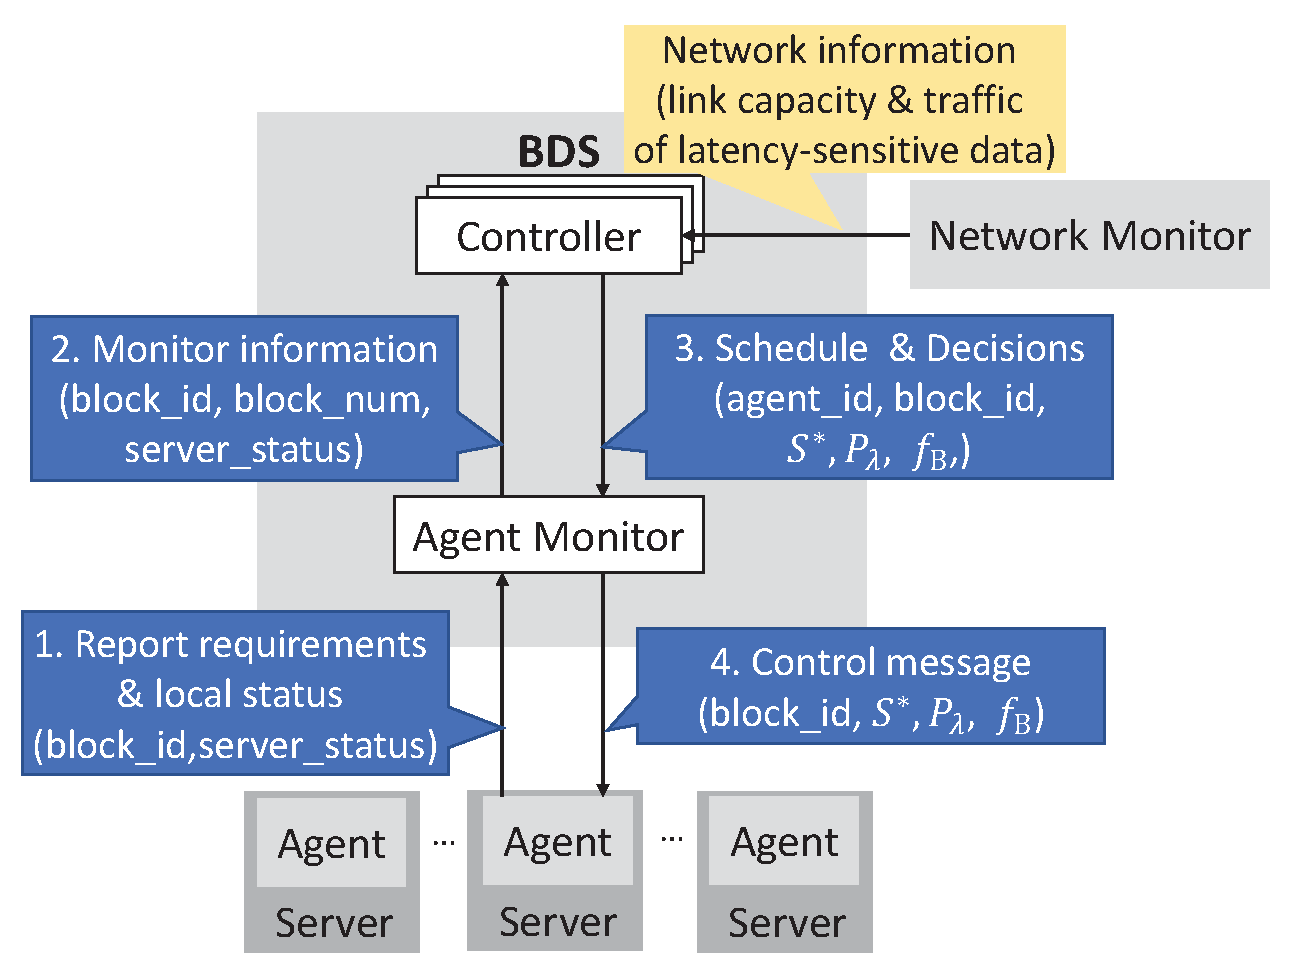
\includegraphics[width=3in]{images/implementation_v2.eps}
  \tightcaption{The system design of \name.}% \jc{where are servers? avoid notions never defined before like "task announcement"}
  \label{fig:implementation}
\vspace{-0.4cm}
\end{figure}
%\vspace{-15pt}

\name takes advantages of the underlying multicast system and the detailed architecture is shown in Figure \ref{fig:implementation}. It consists of four components: Controller, Agent Monitor, Agent, and Network Monitor.
(1) \emph{Controller} runs the centralized scheduling and routing algorithm described in \Section\ref{sec:logic}.
(2) \emph{Agent Monitor} is a messaging layer between \emph{Controller} and \emph{Agents}.
(3) \emph{Agent} is a module running on each server, report local status to the agent monitor, and handles the specific data transfers according to the control messages.
(4) \emph{Network Monitor} monitors the bandwidth used by latency-sensitive traffic and link utilization.

\subsection{Centralized control}
\label{subsec:system:centralized}

The centralized controller of \name sets a 3-second scheduling cycle and updates its decisions at the beginning of each cycle. The control interfaces are implemented by HTTP POST, and include the {\em measurement collection} from agents to the controller, and the {\em control messages} from the controller to agents. Specifically, the basic workflow in one cycle can be described as follows: (1) the local agent on each server checks the block status, records the IDs of blocks that finished downloading in this cycle, and then reports the status and information to the agent monitor; (2) Agent Monitor aggregates the information from all the agents, updates block duplication status and server availability status, and then sends the updated information to the controller; (3) the controller runs the centralized scheduling algorithm, works out the near-optimal scheduling and routing results, and sends them to the agent monitor; (4) agent monitor then forwards the control messages back to the corresponding local agents; finally, (5) the local agent sets the transmission parameters according to the received control message and uses \emph{wget} tools to download the bulk data.
%\jc{the para needs a clearer message: how centralized control is implemented? what's the data collection interface? what's the control interface? Don't use mathmatical notations (again don't assume people have read section 4) or protocols like http post (they belong to implementation).}

There are two optimizations in our implementation.
\begin{itemize}
\item \emph{Blocks merging}.
To reduce the computational scale and achieve higher-efficient transmissions, \name merges the blocks with the same source and destination pair into one subtask.
This has two advantages: (1) it significantly reduces the number of pending blocks in each scheduling cycle, making calculation on the centralized control algorithm computationally more manageable.
(2) it avoids establishing multiple TCP connections between two servers which could cause performance instability and  performance degradation.
%There are two advantages: reducing the computation scale and achieving higher-efficient transmissions. To be specific: 1) there will be a large number of pending blocks in each scheduling cycle, making calculation on the controller computationally hard to finish within an acceptable time, while block merging can significantly reduce the block number and thus reduce the calculation scale; 2) concurrent transmission will make all blocks establish connections at the same time, sharing the limited bandwidth and thus cannot possibly be finished in one cycle. This will result in connection hanging and inefficient transmissions.
\item \emph{Non-blocking update}. While \name centralized algorithm runs several orders of magnitudes faster than traditional technique, it still takes non-negligible amount of time to recalculate the scheduling and routing solutions. To avoid being blocked by the controller decision-making, \name continues the transmissions according to the configurations in the last cycle while waiting for the new configurations. To ensure consistency, the controller estimates the task status at algorithm ending time and uses that estimated status as inputs of the centralized algorithm.
\end{itemize}

%\begin{itemize}
%
%\item Start with the basic workflow of each 3-second cycle: (1) how local agent collects delivery status, (2) send messages to the controller, (3) controller runs the algorithm, (4) control message to each local agent, and (5) how local agent enforce decision.
%
%\item Fault tolerance: what if a server is not available (or straggling), what if one controller instance is not available, what if there is network partition between DCs or between DCs and the controller.
%
%\item Explain two optimizations:
%\begin{itemize}
%\item Merging blocks
%\item Non-blocking update
%\end{itemize}
%
%\end{itemize}

\subsection{Dynamic bandwidth separation}
\label{subsec:system:separation}

%\jc{please mention 80\% utilization upper bound and why the conservative use of bandwidth can protect transient online flows}

To guarantee dynamic bandwidth separation between inter-DC
bulk-data multicasts and delay-sensitive traffic, \name
monitors the aggregated bandwidth usage of all
latency-sensitive flows on each inter-/intra-DC link, and dynamically
calculates the limit on total bandwidth usage of
latency-insensitive inter-DC multicasts every 3 seconds.
Because \name updates routing decision every few seconds,
we reserve 20\% of link capacity to protect online flows
from transient traffic bursts,
%To protect online flows under transient traffic bursty,
%we reserve 20\% link capacity
i.e., the upper bound of the available bandwidth for bulk-data
transfers is set to be the difference between 80\% of
link capacity and the aggregated bandwidth usage of
latency-sensitive traffic.
%With the known link capacity and the aggregated size of latency-sensitive traffic, the residual bandwidth for background data can then be calculated by the difference.

%So that the reserved 20\% link capacity can absorb the traffic jitters, mask the network degradation and ensure the online-server performance. In the server end, each agent enforces the bandwidth limits by Linux Traffic Control (\texttt{tc}). Thus, \name achieves the bandwidth separation dynamically and in real-time.
%\jc{move tc stuff to implementation.}

%Such dynamic bandwidth separation scheme is different from the traditional priority-based techniques (such as \cite{kumar2015bwe}), which sets higher priority to online latency-sensitive traffic than background traffic. When traffic bursts, such priority-based techniques work as usual and allocate bandwidth according to traffic priorities, no matter whether the online traffic is suffering from high latency. As such situation can be avoided in \name, which dynamically monitors the aggregated bandwidth occupied by delay-sensitive applications and reserves enough bandwidth for them, \name guarantees the performance of latency-sensitive applications by leveraging dynamic bandwidth separation.

Based on the dynamic separation, \name's application-level bandwidth allocation scheme in multicast overlay network enjoys two advantages. (1) It uses global coordination to achieve more efficient bandwidth utilization. The traditional priority-based techniques (such as \cite{kumar2015bwe}) that set higher priority to online latency-sensitive traffic than background traffic can not react to the dynamically changing network environment, resulting in bandwidth waste or performance interference. While \name could dynamically monitor the aggregated bandwidth occupied by delay-sensitive applications and reserves moderate amounts of bandwidth for them.
(2) \name is complementary to network-layer techniques that improve the WAN performance. The prior WAN optimization solutions (e.g., traffic engineering studies \cite{chen2012design, kavulya2010analysis, mishra2010towards, reiss2012heterogeneity}) have substantially improved inter-DC applications' performance, while \name's benefits of an application-level overlay network are orthogonal to these works.

%\jc{not sure the logic flows. use this flow instead: (1) bds's app-level bandwidth allocation is complementary to QoS solutions, (2) bds uses global coordination to achieve more efficient bandwidth utilization}

%\jc{please put this solution into context. what's the diff to priority-based techniques such as bwe?}


\subsection{Fault tolerance}
\label{subsec:system:fault}
To make \name fault tolerant, the following scenarios are considered.% and the corresponding evaluations are in \Section\ref{subsubsec:evaluation:adaptability}.

\begin{packedenumerate}
\item \emph{Controller failure:} The controller is replicated for fault tolerance. If the master controller fails, another replica will be elected as the new controller ~\cite{lamport1998part}. If the network partition happens between DCs and the controller, the Agents running in servers will fall back to a default decentralized overlay protocol to ensure graceful performance degradation.
\item \emph{Server failure:} If the agent on this server is still able to work, it will report the abnormal state to the agent monitor. Otherwise, those servers that selected this server as data source would report the unavailability to the agent monitor. In both cases, the controller would remove that server from the potential data sources in the next scheduling cycle.
%\item \emph{What if there is network partition between DCs or between DCs and the controller?} If network partition happens between DCs and the controller, the whole network will fall back to a default decentralized overlay protocol to ensure graceful performance degradation. If network partition happens between DCs, the DCs located in the same partition with the controller will work the same as before, while the separated DCs will fall back to the decentralized overlay network.
\item \emph{Network partition between DCs:}
If network partition happens between DCs, the DCs located in the same partition with the controller will work the same as before, while the separated DCs will fall back to the decentralized overlay network.
\end{packedenumerate}
%
%\begin{itemize}
%
%\item First, how to get real-time aggregated size of latency-sensitive traffic.
%
%\item Second, how to calculate the bandwidth cap for background bulk traffic
%
%\item Finally, how to enforce the bandwidth cap.
%
%\end{itemize}



